%!!!!!!!!!!!!!!!!!!!!!!!!!!!!!!!!!!!!!!!!!!!!!!!!!!!!!!!!!!!!!!!!!!!!!!!!!!!!!!
%!NOTE: This example file has been prepared according to the University of
%!      Hawaii Style & Policy Manual for Theses and Dissertations dated
%!      "Revised September 2010". If you have one with a later date, you may
%!      need to make revisions to this document as well. In any event, making
%!      sure your thesis complies with Graduate Education guidelines is
%!      ultimately your responsibility. Caveat LaTeXtor. :)
%!!!!!!!!!!!!!!!!!!!!!!!!!!!!!!!!!!!!!!!!!!!!!!!!!!!!!!!!!!!!!!!!!!!!!!!!!!!!!!

%% The options are (you can only choose one from each group):
%%
%% 10pt, 11pt, 12pt: chooses the point size for the document. "11pt" is the
%%                   default.
%%
%% oneside, twoside: whether you want your document onesided or twosided. Note
%%                   that twosided is not guaranteed to work, and style
%%                   guidelines prohibit double sided printouts on final
%%                   copy. "oneside" is the default.
%%
%% draft, final: when printing drafts you can save a lot of paper by using the
%%               "draft" option. It switches to single spacing, displays overful
%%               hboxes with a black box, prints a version number on title page 
%%               and omits signature page. Of course for the final copy make
%%               sure to use the "final" option! "final" is the default.
%%
%% thesis, dissertation: switches between the style for a master's thesis and a 
%%                       Ph.D. dissertation. The differences are fairly minor
%%                       and limited to the front matter. "thesis" is the
%%                       default.
%%
%% actual, proposal: switches between actual document and proposal mode. In
%%                   proposal mode: the title page is simplified and the
%%                   version number is always printed.
%%
%%% Load the new uhthesis document class
\documentclass[11pt]{uhthesis}

%%% Load some useful packages:
%% New LaTeX2e graphics support
\usepackage{graphicx}
%% Package to linebreak URLs in a sane manner.
\usepackage{url}

%%% Declarations for Front Matter. Capitalize all of these values
%%% "normally". This allows the document class to format them properly.
%% Full title of thesis or dissertation, capitalized like a title should be.
\title{Neutrino Astrophysics with the ANITA3 Telescope}
%% Your name, capitalized normally. Do not include any titles like Dr.
\author{Benjamin J. Rotter}
%% Month in which you intend to receive your degree (i.e. graduation).
%% Presumably this will be one of: May, August, or December.
\degreemonth{April}
%% Year of expected graduation.
\degreeyear{2016}
%% Type of degree to be conferred.
\degree{Doctor of Philosophy}
%% This is the chairperson of your committee. Do not use titles like Dr.
\chair{Peter Gorham}
%% The other members of your committee, seperated by "\\". Again, no titles,
%% and it is customary to list the outside committee member (if you have one)
%% last.
\othermembers{Gary Varner\\
Bob Morse\\
Jelena Maricic\\
Richard Mills
}
%% The field in which you are obtaining your degree, capitalized normally.
\field{Physics}
%% If your discipline allows subfields, you can add it here. Note that this
%% is strictly controlled, so consult the Style & Policy guide before adding
%% a subfield.
%\subfield{Bioinformatics}
%% 4-6 optional keywords/phrases for use in indexing or as search terms
\keywords{theses, dissertations, graduating, misery}
%% The version number of your document. Consistent use of this will enable you
%% to tell old drafts from new ones. Final actual documents omit this
%% automatically so you can use it without fear of submission problems at the
%% end. If you do not define this parameter, it defaults to "1.0.0".
\versionnum{4.0.0}

%%% End of preamble
\begin{document}
\maketitle

\begin{frontmatter}

%%% Note, there is no longer a signature page included in the document, it
%%% has been replaced by Form IV

%%% Create the copyright page (optional)
%\copyrightpage

%%% Bring in the dedication page from external file (optional)
%%%%%%%%%%%%%%%%%%%%%%%%%%%%%%% -*- Mode: Latex -*- %%%%%%%%%%%%%%%%%%%%%%%%%%%%
%% uhtest-dedication.tex -- 
%% Author          : Robert Brewer
%% Created On      : Fri Oct  2 16:29:01 1998
%% Last Modified By: Robert Brewer
%% Last Modified On: Fri Oct  2 16:29:20 1998
%% RCS: $Id: uhtest-dedication.tex,v 1.1 1998/10/06 02:07:25 rbrewer Exp $
%%%%%%%%%%%%%%%%%%%%%%%%%%%%%%%%%%%%%%%%%%%%%%%%%%%%%%%%%%%%%%%%%%%%%%%%%%%%%%%
%%   Copyright (C) 1998 Robert Brewer
%%%%%%%%%%%%%%%%%%%%%%%%%%%%%%%%%%%%%%%%%%%%%%%%%%%%%%%%%%%%%%%%%%%%%%%%%%%%%%%
%% 

\begin{dedication}
\null\vfil
{\large
\begin{center}
To my family,\\\vspace{12pt}
and my friends,\\\vspace{12pt}
I couldn't have done it without you.
\end{center}}
\vfil\null
\end{dedication}


%%% Bring in the acknowledgments section from external file (optional)
%%%%%%%%%%%%%%%%%%%%%%%%%%%%%%% -*- Mode: Latex -*- %%%%%%%%%%%%%%%%%%%%%%%%%%%%
%% uhtest-acknowledgements.tex -- 
%% Author          : Robert Brewer
%% Created On      : Fri Oct  2 16:29:43 1998
%% Last Modified By: Robert Brewer
%% Last Modified On: Fri Oct  2 16:29:52 1998
%% RCS: $Id: uhtest-acknowledgements.tex,v 1.1 1998/10/06 02:06:54 rbrewer Exp $
%%%%%%%%%%%%%%%%%%%%%%%%%%%%%%%%%%%%%%%%%%%%%%%%%%%%%%%%%%%%%%%%%%%%%%%%%%%%%%%
%%   Copyright (C) 1998 Robert Brewer
%%%%%%%%%%%%%%%%%%%%%%%%%%%%%%%%%%%%%%%%%%%%%%%%%%%%%%%%%%%%%%%%%%%%%%%%%%%%%%%
%% 

\begin{acknowledgments}

	Thank you to everyone who helped me and loved me.

\end{acknowledgments}


%%% Bring in the abstract section from external file
%%%%%%%%%%%%%%%%%%%%%%%%%%%%%% -*- Mode: Latex -*- %%%%%%%%%%%%%%%%%%%%%%%%%%%%
%% uhtest-abstract.tex -- 
%% Author          : Ben Rotter
%% Created On      : Fri Oct  2 16:30:18 1998
%% Last Modified By: Ben Rotter
%% Last Modified On: Fri Oct  2 16:30:25 1998
%% RCS: $Id: uhtest-abstract.tex,v 1.1 1998/10/06 02:06:30 rbrewer Exp $
%%%%%%%%%%%%%%%%%%%%%%%%%%%%%%%%%%%%%%%%%%%%%%%%%%%%%%%%%%%%%%%%%%%%%%%%%%%%%%%
%%   Copyright (C) 1998 Robert Brewer
%%%%%%%%%%%%%%%%%%%%%%%%%%%%%%%%%%%%%%%%%%%%%%%%%%%%%%%%%%%%%%%%%%%%%%%%%%%%%%%
%% 

\begin{abstract}
%Basically here I want to talk about the ANITA3 instrument, the theory that is it stuyding (Cosmogenic neutrinos and cosmic rays), and the results of the recent flight.  I should really mention the link between the cosmic rays (even though it seems like the energies we see are lower than the knee cutoff region) and maybe even add in something about darkmatter strangelets in an appendix or something.  I should probably be doing something to link those two things together


%% This is Ben Rotter, and I'm going to write a dissertation.
%This dissertation is an overview of one experimental study of the highest energy particles created in the cosmos, their propogation through space, and their interaction with other media and subsequent detection on Earth. Ultra-high energy cosmic rays (UHECRs), those with energies on the order of $10^{18}eV$, have been observed colliding with matter in the Earth's atmosphere.  These interactions result in the creation of large, energetic particle showers which can be detected by space and ground based detectors.  Due to the extreme energies of these rare particles, much study was poured into determining their cosmic source accelerator.  From this, precision measurements of the flux density over a wide range of energies have been taken, and several interesting features are found within the spectrum.  Most notibly, at the highest observed energy edge of the spectrum, a sudden decrease in flux (or knee) can be observed.  This energy happens to be situated at a resonance for an interaction between a relativistic particle and the low energy photon background radiation, the CMB.  This interaction involves the creation of a delta resonance whose subsequent decay includes a propagating neutrino.  This highly reletivistic neutrino is hypothesized to have high enough flux to be detectable, and has yet to be observed.  The discovery of this cosminogenic neutrino is the main scope of the ANtarctic Impulsive Transient Antenna (ANITA) telescope payload.  This thesis details the theory, experimental design, and analysis of the third flight of the ANITA experiment, culminating in a defendable limit on the flux density of these mysterious particles, as well as a search for UHECRs.

%% Lets try this again
Ultra-high energy cosmic rays (UHECRs), those with energies above $10^{18}$~eV, have been observed colliding with matter in the Earth's atmosphere by a variety of experiments. These particles are amongst the highest observed locally on earth, with energies many orders of magnitude higher than those produced in terrestrial accelerators.  Due to the extreme energies of these rare particles, much study has been poured into determining their cosmic source accelerator, a search which continues today.  This dissertation explores the third flight of the ANtarctic Impulsive Transient Antenna (ANITA) telescope payload in the 2014-2015 Antarctic season, which has a unique opportunity for novel observations of UHE particles.  It covers the cosmological theory, payload overview, detector calibration, signal simulation, and presents results of measurements of UHECRs and Tau Regeneration UHE$\nu$s with the third ANITA flight.

\end{abstract}


%%% Generate table of contents
%\tableofcontents

%%% Generate list of tables
%\listoftables

%%% Generate list of figures
%\listoffigures

\end{frontmatter}

%\normalsize
%%% Bring in the body of the thesis from external file
%%Below is the guy I stole this template from, because it is great
%%%%%%%%%%%%%%%%%%%%%%%%%%%%%% -*- Mode: Latex -*- %%%%%%%%%%%%%%%%%%%%%%%%%%%%
%% uhtest-body.tex -- 
%% Author          : Robert Brewer
%% Created On      : Fri Oct  2 16:30:37 1998
%% Last Modified By: Robert Brewer
%% Last Modified On: Mon Oct  5 16:01:29 1998
%% RCS: $Id: uhtest-body.tex,v 1.1 1998/10/06 02:07:14 rbrewer Exp $
%%%%%%%%%%%%%%%%%%%%%%%%%%%%%%%%%%%%%%%%%%%%%%%%%%%%%%%%%%%%%%%%%%%%%%%%%%%%%%%
%%   Copyright (C) 1998 Robert Brewer
%%%%%%%%%%%%%%%%%%%%%%%%%%%%%%%%%%%%%%%%%%%%%%%%%%%%%%%%%%%%%%%%%%%%%%%%%%%%%%%
%% 



%%%%%%%%%%%%%%%%%%%%%%%
\chapter{Introduction}
%%%%%%%%%%%%%%%%%%%%%%%

Every dissertation should have an introduction.  You might not realize
it, but the introduction should introduce the concepts, background,
and goals of the dissertation.

\section{Cosmological Theory}
	\subsection{Cosmic Rays}
		The universe is vast and surprising and has just begun to be explored.  As telescopes become larger and more sensitive, we as a species can see further away from our tiny blue speck with increasing clarity.  However, the attenuation of photons in space from fundamental physics interactions clouds the majority of the universe from our gaze.  However, there is a constant flux of bosonic particles incident on earth from various cosmic accelerators.  These messenger particles allow a new window into regions of the universe that were previously inaccessible.  The energy spectrum of these particles introduces an additional mystery, as the sources and interactions of these particles isn't entirely understood.  The makeup of these particles is also poorly understood, whether it be heavy ions or protons.  Additional experimental observations of these cosmological particles will yield a better understanding of both the structure of the matter within the universe at large, as well as fundamental physics processes energetically unachievable from existing collider experiments.  The creation and propagation of ultra high energy cosmic rays through the universe opens a window to understanding of extreme high energy physics.
	\subsection{History}
		Cosmic rays were first observed a century ago, when an unexpected increase in observed bosonic radiation was observed as altitude increased.  Previously, it was expected that radiation was caused by radioactive decays within the earth's crust, however this additional radiative component was indicative of a cosmological source.  This discovery spawned a search for the sources of these particles radiating down from the heavens.
	\subsection{Sources}
		There are numerous cosmic ray sources that have strong theoretical motivation.  Additionally, due to the higher flux of nearby low energy cosmic ray sources, many have gathered experimental evidence to support those theories.  They include such objects and Active Galactic Nuclei (AGN), supernova, quasars, gamma-ray bursts.  However these sources still have uncertainty, and their creation mechanisms may be much more complex than current models suppose.


\section{GZK internation}
		The flux of cosmic ray particles as a function of energy, the energy spectrum.  This spectrum, though quite smooth throughout most, has several characteristic decreases in flux at high energies.  One such flux decrease coincides with the delta resonance rest energy.  This fits nicely with the theory of a relativistic proton colliding with the cosmic microwave background radiation (CMB).  This interaction was predicted by Greisen–Zatsepin–Kuzmin, and represents a theoretical high energy limit on particles coming from outside of the galaxy, known as the GZK limit, at 5x10$^{19}$ eV.  Confoundingly, cosmic ray particles have been observed exceeding this limit, suggesting an intra-galactic source of unknown origin.  The low statistics of particles observed at this energy prevent identification of a specific source.  However, as particles are present at these high energies, it is expected that other regions of the universe also contain accelerators capable of creating cosmic rays in excess of the GZK limit.  The GZK process has multiple channels, neutral current and charged current, each of which produce ultra high energy neutrino messenger particles that can be detected on earth.

\subsection{Neutrino detection on earth}
		Cosmologically propagating neutrinos have an extremely small cross section, such that their path length through empty space is essentially infinite.  This yields a messenger particle that can transmit information about ultra high energy cosmic ray quantity, flux, and energy from regions of the universe not probe-able by classical photon telescopes.  Neutrino telescope observations have been carried out at lower energies for nearly a century, with a recent increase in energies and scale in the past few decades.  Since the term "cosmic ray" describes any high energy particle incident on earth (including gamma rays).  For the purposes of this dissertation, neutrinos fit the description of cosmic rays.
	\subsection{Neutrino hadronic interactions}
		Though neutrinos have a small cross-section with vacuum, they have a non-trivial cross-section with hadronic matter through the weak interaction.  Luckily, the earth where we reside is an enormous target for these low flux particles.  These interactions create a hadronic shower, one that radiates heavily.


%%%%%%%%%%%%%%%%%%%%%%%%%%
\chapter{ANITA Telescope}
%%%%%%%%%%%%%%%%%%%%%%%%%%
\section{Overview}
	The ANITA telescope platform is, in essence, a passive broad-band radio frequency electromagnetic field transient detector and time domain digitizer.  The main structure consists of a collection of radially positioned, outwardly facing, broad-band, highly-directional quad-ridge horn antennas.  The antennas are separated into three different rings, with each ring separated into 16 different "phi-sectors."  This yields several (2-3 for ANITA2, 3 for ANITA3) antennas pointing in the same direction with a physics baseline offset between them. These antennas' feeds are filtered and amplified by a series of low noise-figure signal-chain components, discussed later, before being digitized by custom on board high-speed digitizer chips and readout electronics.  The digitization is triggered on-board, with a separate square-law integrating power detector before being read out to on board redundant data storage.  The payload is capable of reading out ~50Hz of full payload waveforms with low (\textless 5\% ) deadtime to disk through a CPCI interconnect backplane.  Additional position and orientation data is also recorded, as well as multiple diagnostic and in-situ relevant physics measurements.	
	
\section{Quad Ridge Horn Antennas}
	The ANITA instrument utilizes dual polarized quad ridge horn antennas to convert the electromagnetic field incident to the payload into an electrical signal that can be digitized and stored for later analysis.  The main requirements of the antennas are: equal sensitivity over a large range of frequencies, high directionality in order to reduce noise from other RF power sources, dual polarizations with co-located phase centers, low dispersion, and light weight.  \\
	Antennas are located to maximize baseline distance between pairs pointing to similar regions of sky in order to maximize angular resolution recovered from interferometric pointing.  Each successive ANITA flight has added additional antennas to the nadir ring in order to increase the number of baselines, as well as provide an additional $\frac{1}{\sqrt{N}}$ noise reduction for coherently summed waveforms.  The total size of the antennas are dictated by the minimum desired frequency (f=1/$\lambda$), a term dominated by both physical payload constraints as well as anthropogenic CW noise.  Additionally, dual polarizations are required for the physics of the instrument, as the radiation emitted by particle interactions is expected to be radially polarized around the shower axis.  The polarization convolved with the refractive index of the ice will yield an entirely vertically polarized field transient at the payload for shower interactions within the ice, and an entirely horizontally polarized transient for showers above the ice.  The dispersion of the antennas must also be low as the digitization window is small and the square-law power trigger is dependent on all power being within its integration window. \\
	Calibrations of the antennas was performed over a wide range of angles in order to determine the full beam-pattern of the horns in both the E-field and B-field for each polarization.  These measurements were taken for the boresight of every antenna as well, in order to determine stability of the manufacturing process.  These variations are discussed later in the Calibration chapter.
	\subsection{Antenna Theory}
		Since this is my dissertation, I should probably talk a bit about antenna theory and antenna height and stuff like that.  I can either do that here or in the calibration section, but since I'm not very good at that stuff I'll wait.
	
\section{Filtering}
	\subsection{Importance}
		The radiative Askaryan signal has a very wide bandwidth, however there are a few considerations that require the signals read by the ANITA telescope to be limited to a specified bandwidth.  \\
		At the high frequency end of the spectrum, above 1.2GHz, the radiative particles in the shower begin to be resolvable, leading to a loss of coherence of the radiated power.  This is especially true at postions not at the Cherenkov angle from the shower axis.  The lack of coherent signal power in the UHV region, coupled with the increased noise induced from widening the band, advises a low-pass filter on the input of the system. \\
		On the low frequency end, the radiated power from the shower is expected to be both coherent and strong, however the physical limitations of building a long wavelength antenna coupled with the high utilization of the VHF band by radio transmitters on satellites and ground stations lead to a requirement that lower frequencies be removed. \\
	\subsection{Technical Details}
		This band pass filtering is done in two stages, one immediately after the antenna, before the pre-amplifier, in order to prevent saturation of the pre-amplifier from out of band signals.  This filter must have an extremely low in-band loss, as any loss introduced by the filter is gained in full system noise temperature, a value which is cascaded through the entire amplification chain.  This was accomplished with a custom made LARK band pass filter.  The second is done after the full amplification chain in order to remove the added out of band electronic amplifier noise introduced from the system.  This was accomplished with two separate low-pass/high-pass filters.
		
		
\section{Amplification}
	\subsection{Expected Power}
		The power of an Askaryan signal from the continent is proportional to the energy of the incident cosmic ray particle.  The 
	\subsection{Noise Figure} 
	The extremely low signal power of an Askaryan pulse necessitates a minimum of additional electronics noise from the detector.  Besides a background of thermal noise, the dominant continuous noise source is electronics noise from the amplifiers.  This noise is a byproduct of the non-ideal coupling of the amplifier to the input signal that results in the amplification of internal thermal noise seen as a resistance on the front of the amplifier.  The noise figure is increased by any loss of power in front of the amplifiers.  Since the noise figure cascades through an amplifier chain, it is imperative to reduce any additional noise figure at the front of the signal chain, and less important in the subsequent amplifiers.
	
	\subsection{Dynamic Range}
	The various electronics sampling the electric charge on the signal line has a readable value.  This value defines the dynamic range of the system.  Each signal path has its own dynamic range.
	
\section{Digitization}
	The electric field variations incident as a function of time is digitized using an array of fast analog to digital converters (ADCs), custom designed application specific integrated circuits (ASICs).  The ANITA3 instrument utilizes a LABRADOR (Large Analog Bandwidth Recorded And Digital Ordered Readout) chip, designed by Gary Varner.  It is a 12-bit, 2.4GS/s, 256 sample long ADC, yielding a window size of ~100ns.  This is accomplished with a sample and hold ring buffer read out with a wilkinson clock comparing the stored charge in a storage capacitor against a ramp signal driven by a constant current source.  Each chip receives 8 RF analog inputs, as well as a 9th clock channel coincidently propagated to all LAB chips.  The SURF (Signal Unit for Radio Frequency) Board consists of 4 LABRADOR chips in order to create a buffer for continuous sampling.  
	\subsection{Limitations}
	After a hold is issued to a chip, the digitization freezes the ring buffer and yields the chip unable to sample until readout is complete, a process that can take ~1us. \\
	The analog bandwidth of the LAB3B (used in the ANITA3 and ANITA2 experiments) did not fully cover the full bandwidth of the antennas and signal chain due to coupling into the chip through the bond wires in the package.  This yields a drop-off in sensitivity to high frequency signals. \\
	The time between samples is controlled by a charge starved transistor chain that controls the connection between the sampling capacitor and the input RF signal.  Due to process inconsistencies in the manufacturing of the ASICs, the timing between subsequent samples is not well controlled.  This yields a variable delta T that needs to be corrected in calibration of each chip individually.  In addition, it leads to an unevenly sampled time domain waveform, which introduces a difficult to correct frequency response, and requires interpolation between points before creating interferometric maps.  This is processing intensive, an issue that makes doing on board interferometry difficult.
	\subsection{Impulse Response}
	The filtering and amplification chain has a dispersive effect on the signal, which requires a calibration of the system impulse response in order to fully understand the incident electromagnetic field.  An impulse response is the reaction of the system to a brief input signal.\cite(something) This impulse response phase shifts different frequencies of the signal which causes the signal power to be temporally spread.  As correlation between channels is dependent on the full complex parameters of the signal, significant differences between channels will cause a mismatch in digitized correlation even if a coherent electromagnetic impulse was present at the antennas.  \\
	The impulse response was measured by comparing the pulse at the input of the full signal chain to that digitized by the LABRADOR chips, then using Fourier deconvolution to determine the introduced gain and phase offsets.  Though Wiener 
	
	
	
	\subsection{Future development}
	Since the LAB3B was developed in 2005, there has been significant development in the LABRADOR architecture.  The current generation of chip, the LAB4D, is a single channel readout that improves upon the previous generations by both vastly increasing the storage buffer through use of a Storage Capacitor Array (SCA) to increase the record length or buffer depth of the chip.  It also allows for the correction of dT offsets iteratively onboard the chip, minimizing the requirement for post-digitization correction of the waveform.
	
			
		
\section{Triggering}
	As the time domain digitization window is extremely small (100ns is one ten millionth (1e-7) of a second), it is necessary to selectively trigger on segments of time that have a high probability of containing a signal event.  The physics signal created by a UHE particle interaction within the field of view of, and directed towards, the instrument exhibits itself as a picosecond duration high electrical potential emanating from a specific direction.  The background is random incoherent thermal noise or single band constant power anthropogenic sources.  Thus, the triggering system must group together information from several RF channels without full digitization and form a decision before the waveform is overwritten in the ring buffer of the LABRADOR digitizer.  For the ANITA3 system, these triggering decisions were made in the TURF (Triggering Unit for Radio Frequency), which received L1 trigger time and antenna information from the SURFs through the CPCI backplane passthrough connectors.
	\subsection{SHORT square-law power integrator}
		A solution to triggering employed in many RF transient detector experiments is to utilize a square-law integrating power detector.  An Ezaki diode (or tunnel diode), is a nonlinear semiconductor circuit that, in a specific input power region, essentially rectifies and integrates an incoming RF signal through the quantum mechanical effect of electron tunneling.  The diode is capable of taking the extremely fast impulsive signal, with a pulse width of under 1ns, and distributes the power over a longer time scale while simultaneously increasing the signal to noise power ratio.  This allows a clocked comparator circuit, usually running with a max of 4ns/cycle, to latch a electrical signal that crosses a certain threshold.  These L1 triggers can be tuned to a reasonable rate, the specifics of which is detailed below, by altering the comparison voltage with an on board DAC, and each channel can be kept running at a similar rate with a PID loop.  Comparing the timing of these "L1" triggers between antennas with similar pointing directions allows a massive decrease in overall trigger rate dictated by combinatorics.
	\subsection{Tiggering efficiency and quality}
		The trigger must make a trade off between efficiency, the ratio of signals selected for digitization over the total number of signals incident on the detector, and quality, the ratio of the number of true signal event over total selected events.  This trade off is a function of the total maximum readout rate for the detector, which both puts a maximum limit on the number of events capable of being detected, and is related directly to the dead time, the time where the detector is unable to observe an event.  As an example, if the trigger constantly selected all moments in time it would be perfectly efficient, but the quality of the signal would be horrific.  Inversely, if the trigger was set to have perfect quality and only select extremely high power impulsive events, it would have horrible efficiency.  The efficiency of the detector can be statistically measured by injecting signals of varying signal to noise ratio (SNR) at a known rate and observing the rate of measured signals.  This will produce a curve (as seen in a plot I will add) which has a characteristic shape, of which the 50\% efficiency point is the defining metric.  This point will be directly related to the allowable incidental noise trigger rate, which was decided to be set at a rate where the payload would be "dead" for approximately 5\% of the time.  I have to add plots for these things!
	\subsection{Optimization and challenges}
		What little room lies in optimizing the SHORT circuit is entirely in tuning the input power to the tunnel diode circuit.  The inverse-resistance region, where a decrease in voltage yields an increase in current flow, is the primary region where additional input power yields an output that is a square of the input.  This occurs at an extremely low power level, much below the minimum quantization level of the LABRADOR ADC, and thus the power must be attenuated in the signal chain after the split between the trigger and digitizer paths.  In addition, the output power of a fully optimized tunnel diode circuit is extremely small,	requiring amplification to produce a working range for the comparator circuit commensurate to the output of a DAC.  The resolution ( (trig rate)/(DAC count) ) dictates the stability of the trigger system.  If this value is too high, changing the trigger threshold setting for a specific channel would cause a large jump in the overall trigger rate of the system, and possibly allow a channel to dominate (or be excluded from) the global triggers.
	\subsection{Delayed trigger windows for offset baselines}
		As the physical offsets between the rings of antennas exceeds one clock period for most of the angles of interest, it is possible to require a timing separation between the arrival of pulses between the separate antennas.  This modification, made between the ANITA2 and ANITA3 flights, decreases the incidental rate of the trigger, increasing the quality, while maintaining the signal rate and efficiency.  The end result of this (and actually what was done exactly) needs to be written up here, but I'm not sure anyone actually knows!  In the end I think what happens is that a threshold crossing in the bottom rings opens a gate in the upper rings in which a threshold crossing will trigger the full system.  It has the unfortunate side effect of allowing the top ring of antennas to unfairly bais the system, as a noise event there is more likely to trigger the system.  I need to detail this better though.
	\subsection{Phi Sector Masking}
		In the ANITA1 flight, it was discovered that noise sources on the continent had the capability to effectively blind the entire payload during periods when only one side of the payload observes significant noise.  To alleviate this issue, a system where an antenna or collection (phi sector) of antennas experiences a comparative increase in trigger rate in comparison to the rest of the payload, it will be excluded from forming the global system trigger.  This allows the instrument to continue observing quiet areas of the continent and increasing the total livetime of the system.  There are additional nuances to this subsystem, including the possibility of very high power noise (or signal) events continuing to leak into the back and side lobes of the antennas from non-masked phi sectors, that need to be taken into account when making a measurement of the total instrumented area for a flight.
		
	\subsection{Removal of banded trigger in ANITA3}
		The ANITA2 instrument separated each signal channel into 3 frequency sub-bands and one full banded trigger within the SHORT boards, before the tunnel diodes.  The reasoning for this was that neutrino signals are full band; a signal with power dominating a single band would be enough to disqualify an event from being a true signal event.  The requirement for a global trigger was several (how many?) bands, in addition to the full band.  It was decided after the flight that this did not did not decrease the quantity of triggers by a significant amount, and the banding scheme was removed in favor of accommodating additional channels (ANITA2 did not trigger on Hpol and had 8 less antennas than ANITA3, so 56 additional trigger channels were required).  This had the unwanted effect of allowing CW signals from northern satellites to overwhelm the detector during the ANITA3 flight.
		
\section{Power Monitor}
	The second digitization of the RF signal was done by a RF power detector circuit.  The fast waveform data only provides 100ns of unbiased noise data per second (the software trigger paired with the gps trigger, discussed later), so a monitor that digitized a larger fractional percentage of time was desired.  This was accomplished on the SURF board using a commercial RF power monitor IC that converted the RMS voltage of the input signal into a log-magnitude proportional DC output that was digitized by an ADC and read out with the slow read out housekeeping data.  This system, and the additional physics it provides is discussed at length in appendix A.
	
\section{GPS tracking and orientation sensors}
	Since the payload is attached to a free rotation balloon, the orientation and location of the payload was completely uncontrolled and thus needed to be constantly monitored.  This was primarily accomplished with two co-located ADU5 GPS heading receivers in conjunction with a single G12 GPS system.  These 9 GPS antennas, read out once a second, provide a constant update for the location and orientation of the payload with a resolution of a fraction of a degree.
	\subsection{Magnetometer}
		In addition to the heading information provided by the GPS systems, a magnetometer was attached to the payload and used to measure the vector components of the magnetic field throughout the flight.  This system, coupled with a model for the geomagnetic field, could be used as a functional compass assuming an accurate position.  John Russell did a lot of work on this, like a whole summer of work, so I can summarize his work here (and cite him or something).
	\subsection{Sun Sensors}
		Many space borne experiments that require very high pointing and location precision, however are above the altitude where GPS has significant accuracy (is this a thing?), use star sensors to orient themselves.  ANITA's flight path over Antarctica during the austral summer, specifically the continual daylight, is able to use just one star to obtain accurate heading information.  With an accurate time and knowledge of the earth's rotation around the sun, one can use a simple pinhole camera and the four mounted angular sun sensors to determine the heading information for regions of time when the GPS is unavailable or unreliable.
		
\section{CPU, CPCI, and Data Readout}
	The custom LABRADOR digitizer ASICS and various control and command FPGAs are located on custom designed printed circuit boards (PCBs) connected to a central processing unit (CPU) over a compact peripheral component interconnect (cPCI) bus interface.  
	
\section{Data Storage and Telemetry}
	The most important piece of any experiment is the storage of the measurements for later analysis.  The quantity of data taken during flight saturates the hard-linked digital hardware used to read it out and store it, and thus it is not feasible to downlink the entirely of the stored information during flight.  This necessitates the recovery of the payload, or at least the storage vaults, immediately preceding the flight.

	\subsection{Redundant data storage}
		The storage requirements for the flight were met by three separate and unique digital storage formats.  This redundancy ensured that even in the event of a single failure the data from the flight would be preserved.  The first storage method was two identical Helium filled conventional spinning hard disk drives written to by the flight CPU over SATA.  The second method was a separately housed array of six solid state drives written to by a dedicated single board computer which received the flight data over an Ethernet link.  The third storage method, which ended being flown in an inactive state, was the RIFFRAFF handheld flash drive array; a complex system of microcontroller steered multiplexed commercial USB flash drives visible to the flight CPU.  During flight, a failure of the Ethernet link lead to the loss of the SSD array subsystem, leaving only the He Drive storage format intact.  Both drives survived the flight however, and two identical copies of data were recovered.
	
	\subsection{Telemetry}
		Iridium, Openport, TDRSS.  Data and control mentioned here too?
		
	\subsection{GPU prioritization}
		The data limitations of the various telemetry downlink systems allow only a fraction of the total data rate to be transmitted.  This limitation infers a prioritization system in order to only send down events that pass a limited set of post-digitization analysis cuts.  This would allow a limited set of analyzable signals in the event of a catastrophic system failure or recovery.
			
%%%%%%%%%%%%%%%%%%%%%%%%%
\chapter{Instrument Calibration}
%%%%%%%%%%%%%%%%%%%%%%%%%%
\section{Instrument Calibration}
	The values read out by the ADC are related to the electromagnetic plane wave incident on the payload, however to calculate it all channels need to be individually corrected for the response of the system.  This correction will give us a physical measurement that can be compared against simulation of the physical shower interaction in the atmosphere or ice, and its propagation through the intervening medium between the shower core and the payload.
	\subsection{LABRADOR voltage}
		The LAB3 ASCIC uses a ring buffer storage capacitor array (SCA) to store a time series of voltages arriving at the chip, before being digitized with a wilkinson clock and ramp signal comparator coupled system.  The digital value read out by the acquisition software is actually measuring a time between when the ramp signal begins, and when it passes the stored charged in the storage capacitor.  This value must therefore be converted into a voltage that can be propagated back through the signal chain and inform us on the induced potential on the antenna fins.  For this, a pulse was measured immediately before entering the SURF RF input, and then compared against the pulse read out by the acquisition software.
	\subsection{LABRADOR time}
		The LAB3's storage capacitors are controlled by a series of starved transistors which causes each cell to be periodically and sequentially connected to the input signal.  This input controller (name?) is effected by non-idealities of the ASIC manufacturing process and thus do not 

	\subsection{Antenna location photogrammetry}

	\subsection{Phase center optimization}
		The electrical center-point of the antennas, though directly related to the physical position and orientation of the antenna, requires an additional calibration.  The phase center, or point at which the electromagnetic field couples to the antenna and begins propagating through the signal cables, is a function of frequency and incident wave direction, so the calibration must consider a large phase space.  The calibration measurements are done in-situo by a ground pulser at WAIS divide sending a pulse to the payload as it passes overhead.  This pulse can be used to determine  the relative phase center offsets between nearby antennas.  The positional error of the phase centers relates directly to the pointing error for events seen later in the flight.





%%%%%%%%%%%%%%%%%%%%%%%%%%
\chapter{Analysis of ANITA3 flight data}
%%%%%%%%%%%%%%%%%%%%%%%%%%
\section{Overview}
	The data recorded by the ANITA3 flight instrument requires a significant analysis effort to extract a meaningful physics result.  In our case, we need to use the raw digital values read out for each channel to determine the analog electromagnetic environment surrounding the payload during brief moments the trigger system determined a physics event may be occurring.  From this, we can use an understanding of the physical geometry of the antennas mounted on the payload, including their orientation and electrical responses, to determine the cause of any incident wave patterns read out by the digitizers.  Once these wave patterns are identified and classified, they can be sorted into signal and background thermal or anthropogenic noise sources via a series of procedural cuts.  This section details the process and results of this analysis.
	

\section{De-dispersion}
		
	
\section{Constant wave source filtering}

\section{Known object categorization}

\section{Interferometric pointing}

\section{Thermal noise cuts}

\section{Polarization cuts}

\section{Base and non-base clustering}


	
	

%%%%%%%%%%%%%%%%%%%%%%%%%%
\chapter{Simulation and expected event rate from analysis techniques}
%%%%%%%%%%%%%%%%%%%%%%%%%%
\section{Overview}
	The series of analysis procedures used to categorize events into signal and noise boxes
	
			
			
			
			
			
			
%%%%%%%%%%%%%%%%%%%%%%%%%%%		
\chapter{Appendix A}
%%%%%%%%%%%%%%%%%%%%%%%%%%%
\section{Overview}
	This appendix deals primarily with the detection of Anti-Quark Nuggets, an exotic dark matter candidate particle, using the ANITA power monitor subsystem.
	
	
	
	
	
	
	
%%%%%%%%%%%%%%%%%%%%%%%%%%%%%%%%%%%%%%	
%\chapter{Examples of LATEX stuff}
%
%%% Here is an example of how to create a floating table. Note that the caption
%%% occurs _before_ the table, unlike a figure where it appears after!
%%%
%%% The "[htbp]" allows the table to be placed: here, top of page, bottom of
%%% page or on a seperate floats page, whatever works best.
%\begin{table}[htbp]
%  %% If you have a really long caption, you can enclose a short version for the
%  %% the List of Tables in "[]", and the full caption in "{}" as we do here
%  \caption[A normal size table.]{A normal size table. There has been a complaint
%    that table captions are not single-spaced, but they should be. This is a
%    test of that feature.}
%  %% This label allows references from other parts of the text to be
%  %% automatically calculated. Labels usually start with three letters
%  %% describing what is being tabled followed by a colon. This prevents label
%  %% mixups. Note that the label must follow the caption for proper numbering.
%  \label{tab:example-1}
%  \begin{center}
%    \begin{tabular}{|l|r|}
%      \hline 
%      Title & Author \\
%      \hline
%      War And Peace & Leo Tolstoy \\
%      The Great Gatsby & F. Scott Fitzgerald \\ \hline
%    \end{tabular}
%  \end{center}
%\end{table}
%
%\chapter{Previous Work}
%
%Some other research was once performed. You can check out a beautiful picture
%in figure \ref{fig:example-1}.
%
%%\begin{figure}[htbp]
%%  \centering
%%  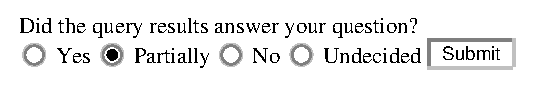
\includegraphics{example-figure.eps}
%%  \caption{An example of included Encapsulated PostScript (EPS).}
%% \label{fig:example-1}
%%\end{figure}
%
%\section{URLs}
%In this modern age, you may find that you wish to include URLs or pathnames
%which both tend to be long and hard for TeX to deal with because it doesn't
%know where to insert linebreaks. The ``{\tt url}'' package (loaded in the main
%uhtest.tex file) allows one to deal with these URLs. For example:
%
%Here is an URL which cannot be broken, leading to terrible output
%$<$http://www.hotwired.com/webmonkey/98/16/index2a.html$>$
%%% The "<>" have to be entered in math mode, that's where the "$"s come from.
%
%Using the package we get the much nicer \url{<http://www.hotwired.com/
%webmonkey/98/16/index2a.html>} which LaTeX can handle just fine. Even better,
%the parameter to {\tt $\backslash$url} can have spaces inserted anywhere so you
%can make the LaTeX source lines in your text editor wrap nicely.
%
%A few notes. It is recommended that you enclose your URLs in ``$<>$'' to ensure
%that any punctuation around the URL won't be confused as part of the URL. You
%can use URLs in your bibliography too (see the {\tt uhtest.bib} file for an
%example). Finally, if you need to use a tilde in your URL then things are a
%little trickier. One way to do it is like this:
%\url{<http://www.dartmouth.edu/}$\sim$\url{jonh/ff-cache/1.html>}. The {\tt
%$\backslash$url} style uses math mode internally, so we break the URL into two
%pieces, and stick a tilde from math mode inbetween the two parts.
%
%\section{Bibliography Citations}
%Citing references to your bibliography is easy \cite{lamport:latex}
%\cite{patashnik:bibtex}. First you build a BibTeX file which contains the
%records for all of the works you wish to cite. This file ends with a ``{\tt
%.bib}'' extension. Then in your body you use the ``{\tt $\backslash$cite}''
%command with the label you gave to the record in question. The final steps are: 
%run LaTeX once, run BibTeX, and then run LaTeX twice more. You should now have
%a bibliography that includes those citations.
%
%\chapter{Conclusion}
%
%This is going to be the chapter where I check the length of the page to make
%sure the bottom margin works out all right.  I hope you don't mind long
%annoying and useless paragraphs because you are sure to get a lot of them here!
%
%\section{Widgets}
%
%This is going to be the chapter where I check the length of the page
%to make sure the bottom margin works out all right.  I hope you don't
%mind long annoying and useless paragraphs because you are sure to get
%a lot of them here!
%
%\subsection{Sub-Widgets}
%
%This is going to be the chapter where I check the length of the page
%to make sure the bottom margin works out all right.  I hope you don't
%mind long annoying and useless paragraphs because you are sure to get
%a lot of them here!
%
%\subsubsection{Sub-Sub-Widgets}
%
%This is going to be the chapter where I check the length of the page
%to make sure the bottom margin works out all right.  I hope you don't
%mind long annoying and useless paragraphs because you are sure to get
%a lot of them here!
%
%\paragraph{Para-Widgets}
%
%This is going to be the chapter where I check the length of the page
%to make sure the bottom margin works out all right.  I hope you don't
%mind long annoying and useless paragraphs because you are sure to get
%a lot of them here!
%
%\subparagraph{Sub-Para-Widgets}
%
%This is going to be the chapter where I check the length of the page
%to make sure the bottom margin works out all right.  I hope you don't
%mind long annoying and useless paragraphs because you are sure to get
%a lot of them here!
%
%This is going to be the chapter where I check the length of the page
%to make sure the bottom margin works out all right.  I hope you don't
%mind long annoying and useless paragraphs because you are sure to get
%a lot of them here!
%
%This is going to be the chapter where I check the length of the page
%to make sure the bottom margin works out all right.  I hope you don't
%mind long annoying and useless paragraphs because you are sure to get
%a lot of them here!
%
%This is going to be the chapter where I check the length of the page
%to make sure the bottom margin works out all right.  I hope you don't
%mind long annoying and useless paragraphs because you are sure to get
%a lot of them here!
%
%This is going to be the chapter where I check the length of the page
%to make sure the bottom margin works out all right.  I hope you don't
%mind long annoying and useless paragraphs because you are sure to get
%a lot of them here!
%
%This is going to be the chapter where I check the length of the page
%to make sure the bottom margin works out all right.  I hope you don't
%mind long annoying and useless paragraphs because you are sure to get
%a lot of them here!
%
%This is going to be the chapter where I check the length of the page
%to make sure the bottom margin works out all right.  I hope you don't
%mind long annoying and useless paragraphs because you are sure to get
%a lot of them here!
%
%This is going to be the chapter where I check the length of the page
%to make sure the bottom margin works out all right.  I hope you don't
%mind long annoying and useless paragraphs because you are sure to get
%a lot of them here!
%
%This is going to be the chapter where I check the length of the page
%to make sure the bottom margin works out all right.  I hope you don't
%mind long annoying and useless paragraphs because you are sure to get
%a lot of them here!
%
%This is going to be the chapter where I check the length of the page
%to make sure the bottom margin works out all right.  I hope you don't
%mind long annoying and useless paragraphs because you are sure to get
%a lot of them here!
%
%This is going to be the chapter where I check the length of the page
%to make sure the bottom margin works out all right.  I hope you don't
%mind long annoying and useless paragraphs because you are sure to get
%a lot of them here!
%
%This is going to be the chapter where I check the length of the page
%to make sure the bottom margin works out all right.  I hope you don't
%mind long annoying and useless paragraphs because you are sure to get
%a lot of them here!
%
%This is going to be the chapter where I check the length of the page
%to make sure the bottom margin works out all right.  I hope you don't
%mind long annoying and useless paragraphs because you are sure to get
%a lot of them here!
%
%This is going to be the chapter where I check the length of the page
%to make sure the bottom margin works out all right.  I hope you don't
%mind long annoying and useless paragraphs because you are sure to get
%a lot of them here!
%
%This is going to be the chapter where I check the length of the page
%to make sure the bottom margin works out all right.  I hope you don't
%mind long annoying and useless paragraphs because you are sure to get
%a lot of them here!
%
%This is going to be the chapter where I check the length of the page
%to make sure the bottom margin works out all right.  I hope you don't
%mind long annoying and useless paragraphs because you are sure to get
%a lot of them here!


%%% Switch to appendix mode
%\appendix

%%% Bring in any appendices from external file (optional)
%%%%%%%%%%%%%%%%%%%%%%%%%%%%%%% -*- Mode: Latex -*- %%%%%%%%%%%%%%%%%%%%%%%%%%%%
%% uhtest-appendix.tex -- 
%% Author          : Robert Brewer
%% Created On      : Fri Oct  2 16:31:12 1998
%% Last Modified By: Robert Brewer
%% Last Modified On: Mon Oct  5 14:41:05 1998
%% RCS: $Id: uhtest-appendix.tex,v 1.1 1998/10/06 02:07:03 rbrewer Exp $
%%%%%%%%%%%%%%%%%%%%%%%%%%%%%%%%%%%%%%%%%%%%%%%%%%%%%%%%%%%%%%%%%%%%%%%%%%%%%%%
%%   Copyright (C) 1998 Robert Brewer
%%%%%%%%%%%%%%%%%%%%%%%%%%%%%%%%%%%%%%%%%%%%%%%%%%%%%%%%%%%%%%%%%%%%%%%%%%%%%%%
%% 

\chapter{Some Ancillary Stuff}

Ancillary material should be put in appendices, which appear before the
bibliography. 

\chapter{More Ancillary Stuff}

Subsequent chapters are labeled with letters of the alphabet.


%% Just for demo purposes, include all entries from bib file
%\nocite{*}

%%% Input file for bibliography
%\bibliography{example}
%% Use this for an alphabetically organized bibliography
%\bibliographystyle{plain}
%% Use this for a reference order organized bibliography
%\bibliographystyle{unsrt}

\end{document}
